\documentclass[conference]{IEEEtran}
\usepackage[T1]{fontenc}
\usepackage{amsmath,amssymb}
\usepackage{graphicx}
\usepackage{booktabs}
\usepackage{multirow}
\usepackage{xcolor}
\usepackage{algorithm}
\usepackage{algpseudocode}
\usepackage{hyperref}
\usepackage{cleveref}
% generated by scripts/make_report.py; do not edit
\providecommand{\pending}{\textbf{\textsc{pending}}}
\newcommand{\LLMOnlyIntent}{\pending{}}
\newcommand{\LLMOnlyRcaOne}{\pending{}}
\newcommand{\LLMOnlyRcaThree}{\pending{}}
\newcommand{\LLMOnlyFix}{\pending{}}
\newcommand{\LLMOnlySafe}{\pending{}}
\newcommand{\LLMOnlyOverPriv}{\pending{}}
\newcommand{\LLMOnlyHalluc}{\pending{}}
\newcommand{\LLMOnlyExcess}{\pending{}}
\newcommand{\LLMOnlySec}{\pending{}}
\newcommand{\LLMOnlyRecall}{\pending{}}
\newcommand{\LLMCheckIntent}{\pending{}}
\newcommand{\LLMCheckRcaOne}{\pending{}}
\newcommand{\LLMCheckRcaThree}{\pending{}}
\newcommand{\LLMCheckFix}{\pending{}}
\newcommand{\LLMCheckSafe}{\pending{}}
\newcommand{\LLMCheckOverPriv}{\pending{}}
\newcommand{\LLMCheckHalluc}{\pending{}}
\newcommand{\LLMCheckExcess}{\pending{}}
\newcommand{\LLMCheckSec}{\pending{}}
\newcommand{\LLMCheckRecall}{\pending{}}
\newcommand{\LLMVerifyIntent}{\pending{}}
\newcommand{\LLMVerifyRcaOne}{\pending{}}
\newcommand{\LLMVerifyRcaThree}{\pending{}}
\newcommand{\LLMVerifyFix}{\pending{}}
\newcommand{\LLMVerifySafe}{\pending{}}
\newcommand{\LLMVerifyOverPriv}{\pending{}}
\newcommand{\LLMVerifyHalluc}{\pending{}}
\newcommand{\LLMVerifyExcess}{\pending{}}
\newcommand{\LLMVerifySec}{\pending{}}
\newcommand{\LLMVerifyRecall}{\pending{}}
\newcommand{\RulesIntent}{89.6\%}
\newcommand{\RulesRcaOne}{89.6\%}
\newcommand{\RulesRcaThree}{89.6\%}
\newcommand{\RulesFix}{89.6\%}
\newcommand{\RulesSafe}{89.6\%}
\newcommand{\RulesOverPriv}{0.0\%}
\newcommand{\RulesHalluc}{0.0\%}
\newcommand{\RulesExcess}{0.00}
\newcommand{\RulesSec}{0.1}
\newcommand{\RulesRecall}{89.3\%}
\newcommand{\CMNoLPIntent}{\pending{}}
\newcommand{\CMNoLPRcaOne}{\pending{}}
\newcommand{\CMNoLPRcaThree}{\pending{}}
\newcommand{\CMNoLPFix}{\pending{}}
\newcommand{\CMNoLPSafe}{\pending{}}
\newcommand{\CMNoLPOverPriv}{\pending{}}
\newcommand{\CMNoLPHalluc}{\pending{}}
\newcommand{\CMNoLPExcess}{\pending{}}
\newcommand{\CMNoLPSec}{\pending{}}
\newcommand{\CMNoLPRecall}{\pending{}}
\newcommand{\CMIntent}{\pending{}}
\newcommand{\CMRcaOne}{\pending{}}
\newcommand{\CMRcaThree}{\pending{}}
\newcommand{\CMFix}{\pending{}}
\newcommand{\CMSafe}{\pending{}}
\newcommand{\CMOverPriv}{\pending{}}
\newcommand{\CMHalluc}{\pending{}}
\newcommand{\CMExcess}{\pending{}}
\newcommand{\CMSec}{\pending{}}
\newcommand{\CMRecall}{\pending{}}
\newcommand{\LLMCheckSmallIntent}{\pending{}}
\newcommand{\LLMCheckSmallRcaOne}{\pending{}}
\newcommand{\LLMCheckSmallRcaThree}{\pending{}}
\newcommand{\LLMCheckSmallFix}{\pending{}}
\newcommand{\LLMCheckSmallSafe}{\pending{}}
\newcommand{\LLMCheckSmallOverPriv}{\pending{}}
\newcommand{\LLMCheckSmallHalluc}{\pending{}}
\newcommand{\LLMCheckSmallExcess}{\pending{}}
\newcommand{\LLMCheckSmallSec}{\pending{}}
\newcommand{\LLMCheckSmallRecall}{\pending{}}
\newcommand{\CMSmallIntent}{\pending{}}
\newcommand{\CMSmallRcaOne}{\pending{}}
\newcommand{\CMSmallRcaThree}{\pending{}}
\newcommand{\CMSmallFix}{\pending{}}
\newcommand{\CMSmallSafe}{\pending{}}
\newcommand{\CMSmallOverPriv}{\pending{}}
\newcommand{\CMSmallHalluc}{\pending{}}
\newcommand{\CMSmallExcess}{\pending{}}
\newcommand{\CMSmallSec}{\pending{}}
\newcommand{\CMSmallRecall}{\pending{}}
\newcommand{\OracleIntent}{100.0\%}
\newcommand{\OracleRcaOne}{100.0\%}
\newcommand{\OracleRcaThree}{100.0\%}
\newcommand{\OracleFix}{100.0\%}
\newcommand{\OracleSafe}{100.0\%}
\newcommand{\OracleOverPriv}{0.0\%}
\newcommand{\OracleHalluc}{0.0\%}
\newcommand{\OracleExcess}{0.00}
\newcommand{\OracleSec}{0.1}
\newcommand{\OracleRecall}{99.4\%}
\newcommand{\LLMOnlyIntentFull}{\pending{}}
\newcommand{\LLMOnlyRcaOneFull}{\pending{}}
\newcommand{\LLMOnlyRcaThreeFull}{\pending{}}
\newcommand{\LLMOnlyFixFull}{\pending{}}
\newcommand{\LLMOnlySafeFull}{\pending{}}
\newcommand{\LLMOnlyOverPrivFull}{\pending{}}
\newcommand{\LLMOnlyHallucFull}{\pending{}}
\newcommand{\LLMOnlyExcessFull}{\pending{}}
\newcommand{\LLMOnlySecFull}{\pending{}}
\newcommand{\LLMOnlyRecallFull}{\pending{}}
\newcommand{\LLMCheckIntentFull}{\pending{}}
\newcommand{\LLMCheckRcaOneFull}{\pending{}}
\newcommand{\LLMCheckRcaThreeFull}{\pending{}}
\newcommand{\LLMCheckFixFull}{\pending{}}
\newcommand{\LLMCheckSafeFull}{\pending{}}
\newcommand{\LLMCheckOverPrivFull}{\pending{}}
\newcommand{\LLMCheckHallucFull}{\pending{}}
\newcommand{\LLMCheckExcessFull}{\pending{}}
\newcommand{\LLMCheckSecFull}{\pending{}}
\newcommand{\LLMCheckRecallFull}{\pending{}}
\newcommand{\LLMVerifyIntentFull}{\pending{}}
\newcommand{\LLMVerifyRcaOneFull}{\pending{}}
\newcommand{\LLMVerifyRcaThreeFull}{\pending{}}
\newcommand{\LLMVerifyFixFull}{\pending{}}
\newcommand{\LLMVerifySafeFull}{\pending{}}
\newcommand{\LLMVerifyOverPrivFull}{\pending{}}
\newcommand{\LLMVerifyHallucFull}{\pending{}}
\newcommand{\LLMVerifyExcessFull}{\pending{}}
\newcommand{\LLMVerifySecFull}{\pending{}}
\newcommand{\LLMVerifyRecallFull}{\pending{}}
\newcommand{\RulesIntentFull}{90.6\%}
\newcommand{\RulesRcaOneFull}{90.6\%}
\newcommand{\RulesRcaThreeFull}{90.6\%}
\newcommand{\RulesFixFull}{90.6\%}
\newcommand{\RulesSafeFull}{90.6\%}
\newcommand{\RulesOverPrivFull}{0.0\%}
\newcommand{\RulesHallucFull}{0.0\%}
\newcommand{\RulesExcessFull}{0.00}
\newcommand{\RulesSecFull}{0.1}
\newcommand{\RulesRecallFull}{90.5\%}
\newcommand{\CMNoLPIntentFull}{\pending{}}
\newcommand{\CMNoLPRcaOneFull}{\pending{}}
\newcommand{\CMNoLPRcaThreeFull}{\pending{}}
\newcommand{\CMNoLPFixFull}{\pending{}}
\newcommand{\CMNoLPSafeFull}{\pending{}}
\newcommand{\CMNoLPOverPrivFull}{\pending{}}
\newcommand{\CMNoLPHallucFull}{\pending{}}
\newcommand{\CMNoLPExcessFull}{\pending{}}
\newcommand{\CMNoLPSecFull}{\pending{}}
\newcommand{\CMNoLPRecallFull}{\pending{}}
\newcommand{\CMIntentFull}{\pending{}}
\newcommand{\CMRcaOneFull}{\pending{}}
\newcommand{\CMRcaThreeFull}{\pending{}}
\newcommand{\CMFixFull}{\pending{}}
\newcommand{\CMSafeFull}{\pending{}}
\newcommand{\CMOverPrivFull}{\pending{}}
\newcommand{\CMHallucFull}{\pending{}}
\newcommand{\CMExcessFull}{\pending{}}
\newcommand{\CMSecFull}{\pending{}}
\newcommand{\CMRecallFull}{\pending{}}
\newcommand{\LLMCheckSmallIntentFull}{\pending{}}
\newcommand{\LLMCheckSmallRcaOneFull}{\pending{}}
\newcommand{\LLMCheckSmallRcaThreeFull}{\pending{}}
\newcommand{\LLMCheckSmallFixFull}{\pending{}}
\newcommand{\LLMCheckSmallSafeFull}{\pending{}}
\newcommand{\LLMCheckSmallOverPrivFull}{\pending{}}
\newcommand{\LLMCheckSmallHallucFull}{\pending{}}
\newcommand{\LLMCheckSmallExcessFull}{\pending{}}
\newcommand{\LLMCheckSmallSecFull}{\pending{}}
\newcommand{\LLMCheckSmallRecallFull}{\pending{}}
\newcommand{\CMSmallIntentFull}{\pending{}}
\newcommand{\CMSmallRcaOneFull}{\pending{}}
\newcommand{\CMSmallRcaThreeFull}{\pending{}}
\newcommand{\CMSmallFixFull}{\pending{}}
\newcommand{\CMSmallSafeFull}{\pending{}}
\newcommand{\CMSmallOverPrivFull}{\pending{}}
\newcommand{\CMSmallHallucFull}{\pending{}}
\newcommand{\CMSmallExcessFull}{\pending{}}
\newcommand{\CMSmallSecFull}{\pending{}}
\newcommand{\CMSmallRecallFull}{\pending{}}
\newcommand{\OracleIntentFull}{100.0\%}
\newcommand{\OracleRcaOneFull}{100.0\%}
\newcommand{\OracleRcaThreeFull}{100.0\%}
\newcommand{\OracleFixFull}{100.0\%}
\newcommand{\OracleSafeFull}{100.0\%}
\newcommand{\OracleOverPrivFull}{0.0\%}
\newcommand{\OracleHallucFull}{0.0\%}
\newcommand{\OracleExcessFull}{0.00}
\newcommand{\OracleSecFull}{0.1}
\newcommand{\OracleRecallFull}{99.7\%}
\newcommand{\NTest}{310}
\newcommand{\NSingle}{260}
\newcommand{\NMulti}{50}
\newcommand{\NDev}{88}
\newcommand{\NClasses}{26}
\newcommand{\NTemplates}{5}
\newcommand{\NCandidates}{2934}
\newcommand{\NDropOne}{47}
\newcommand{\NDropFour}{0}
\newcommand{\Agreement}{100.0\%}
\newcommand{\NCore}{154}
\newcommand{\IamFidelity}{\pending{}}
\newcommand{\IamFidelityN}{\pending{}}
\newcommand{\LiveFidelity}{\pending{}}
\newcommand{\LiveFidelityN}{\pending{}}

\newcommand{\sys}{\textsc{CloudMedic}}
\newcommand{\bench}{\textsc{CloudMedic-Bench}}
\newcommand{\todo}[1]{\textcolor{red}{[TODO: #1]}}

\begin{document}
\title{\sys: Verified, Least-Privilege Troubleshooting of AWS Network and IAM Misconfigurations with Language Models and Formal Repair}
\author{\IEEEauthorblockN{Mithin Sagar}\IEEEauthorblockA{Department of Computer Science and Engineering\\ \todo{institution}\\ mithinsagar@gmail.com}}
\maketitle

\begin{abstract}
Cloud support engineers spend much of their time on configuration tickets: an instance that cannot reach a database, a
Lambda function that times out, an \texttt{AccessDenied} that ``should not happen''. Large language models (LLMs) can read
such tickets, but their diagnoses are unverified and their fixes often widen access, for example by opening a security
group to \texttt{0.0.0.0/0} or granting \texttt{s3:*}. We present \sys, a hybrid troubleshooter in which a small local LLM only
translates the ticket into a formal \emph{intent}, while formal models of VPC reachability and IAM policy evaluation find
every failing hop and a counterexample-guided MaxSMT search synthesises the fix that restores the intent with the least
added privilege. To measure this we define \emph{excess privilege}, the network flows and IAM grants a fix creates beyond both
the intended and the pre-fix configuration, and release \bench{}, \NTest{} validated fault-injection scenarios over
\NClasses{} fault classes and \NTemplates{} reference architectures, including \NMulti{} multi-fault cases in which each
fault masks the other. On a stratified \NCore{}-scenario core set, \sys{} with a 7B model produces a working fix with zero excess
privilege and zero regression in \CMSafe{} of tickets, compared with \LLMCheckSafe{} for the same model prompted with an expert
checklist and \LLMVerifySafe{} when that model also receives verifier feedback. We validate the IAM model against the AWS
policy simulator (\IamFidelity{} agreement) and the network model against live probes on AWS (\LiveFidelity{}).
Everything runs on a laptop at zero cost.
\end{abstract}

\section{Introduction}
Configuration mistakes are a frequent cause of cloud access and connectivity problems, and diagnosing them is a large
part of the work of cloud support roles. A typical ticket is short and imprecise (``our app server can no longer reach the
database since last night's deploy'') while the configuration that explains it is large and layered: security groups
(stateful), network ACLs (stateless, ordered), route tables, NAT and internet gateways, peering, private DNS, and for
access problems a stack of identity policies, permissions boundaries, service control policies (SCPs), resource
policies, VPC endpoint policies and KMS key policies, evaluated in a precise order.

LLMs are attractive for this task because tickets are natural language, and recent work applies them to incident root-cause
analysis~\cite{ahmed2023recommending,chen2024rcacopilot}. Two problems remain. First, an LLM diagnosis is a guess: nothing
checks it against the configuration. Second, and less studied, an LLM \emph{fix} can be worse than the fault. A model that
``fixes'' a denied request by granting a service wildcard, or a timeout by opening a port to the internet, closes the ticket
and opens a security incident. Support engineers are expected to resolve tickets without weakening the customer's security
posture, so a useful assistant must be judged on whether its fix is \emph{correct and minimal}, not only on whether it names
the right resource.

AWS already uses automated reasoning to answer \emph{questions} about configurations: Zelkova encodes IAM policies in
SMT~\cite{backes2018semantic} and Tiros answers network reachability queries~\cite{backes2019reachability}. Network
verification more broadly is mature~\cite{kazemian2012hsa,fogel2015batfish}. These tools need a formal query, which customers
do not write, and they report violations rather than synthesising repairs. \sys{} connects the two worlds: the LLM produces
the formal query from the ticket, and formal reasoning does everything that must be right.

\textbf{Contributions.}
\begin{enumerate}
\item \textbf{Executable models} of VPC packet reachability and IAM authorisation for a documented subset of AWS semantics,
with \emph{full-path evaluation} that reports every failing hop, so faults masked by earlier faults remain visible (\cref{sec:models}).
\item \textbf{Least-privilege repair} by counterexample-guided MaxSMT over a typed edit language, with cost equal to the
measured privilege a candidate adds, branch-and-bound over non-additive interactions, and a collateral-damage guard (\cref{sec:repair}).
\item \textbf{The excess-privilege metric} for evaluating configuration fixes, and \bench{}, a fault-injection benchmark whose
labels hold by construction and whose every scenario passes four validity checks (\cref{sec:bench}).
\item \textbf{An evaluation} against LLM-only, checklist-prompted and verifier-feedback baselines, ablations of the cost function
and model size, and fidelity checks of the models against AWS itself (\cref{sec:eval}).
\end{enumerate}
Code, benchmark and all run logs are released. All experiments use open-weight models on a laptop (Apple M5, 16\,GB).

\section{Background and Related Work}
\textbf{LLMs for cloud incidents.} Ahmed et al.\ evaluated LLMs for recommending root causes and mitigations for production
incidents~\cite{ahmed2023recommending}; RCACopilot retrieves diagnostic information and asks an LLM to classify the root
cause~\cite{chen2024rcacopilot}. Benchmarks for AI agents in operations now exist: AIOpsLab~\cite{chen2025aiopslab},
ITBench~\cite{jha2025itbench}, OpenRCA~\cite{xu2025openrca} and RCAEval~\cite{pham2025rcaeval}. They mostly target
microservice application failures observed through telemetry. \bench{} targets the complementary setting of
\emph{infrastructure configuration} faults explained by the control-plane state, and scores fixes, not only localisation.

\textbf{Automated reasoning about cloud configuration.} Zelkova~\cite{backes2018semantic} and Tiros~\cite{backes2019reachability}
answer IAM and network questions with SMT and are used in production AWS features. Batfish~\cite{fogel2015batfish} and header
space analysis~\cite{kazemian2012hsa} verify network configurations. Our models are far smaller in scope; their purpose is to
provide verified obligations and a repair oracle in a closed loop with an LLM.

\textbf{Verification and feedback for LLM output.} Iterative self-refinement~\cite{madaan2023selfrefine} and tool feedback improve
LLM answers, and hallucination is a known failure mode~\cite{ji2023hallucination}. We compare against this design directly: the
\emph{verifier-loop} baseline gives the LLM the same verifier's failing checks and lets it revise its fix twice.

\textbf{Least privilege and mutation.} The principle of least privilege~\cite{saltzer1975protection} motivates our cost function.
Our benchmark construction borrows from mutation testing~\cite{jia2011mutation}: faults are generated by operators applied to
known-good artefacts.

\section{Problem Formulation}\label{sec:problem}
A \emph{snapshot} $S$ is a JSON description of an account's VPCs, subnets, route tables, gateways, peerings, endpoints,
security groups, network ACLs, compute (EC2, Lambda, RDS), private hosted zones, IAM roles and policies, SCPs and resource
policies. An \emph{intent} $\iota$ states what the customer expects to work: either a flow
$(\mathit{src}, \mathit{dst}, \mathit{proto}, \mathit{port})$, where $\mathit{dst}$ may be a DNS name, or a request
$(\mathit{principal}, \mathit{action}, \mathit{resource})$. A ticket $T$ describes a failing intent in natural language.
Given $(T, S)$ a system outputs ranked root causes $(c_k, r_k)$, a fault class from a closed vocabulary of \NClasses{} classes and
the misconfigured resource, and a fix: a list of edits in a typed language of 23 operations (adding a security-group rule,
adding a NACL entry, adding a route, adding or replacing a policy statement, associating a hosted zone, and so on). Edits
that name non-existent resources or are malformed are rejected and counted.

\textbf{Access surface and excess privilege.} For a snapshot $S$ we define its access surface $A(S)$ over a finite universe
fixed per scenario: all flows between compute endpoints and external hosts on a set of commonly attacked ports plus every
listening port, and all (role, action, resource) triples over a 34-action catalogue (16 actions marked sensitive) and all
modelled resources. A flow is in $A(S)$ if the network path permits it, whether or not a service listens, because an open
path is exposure. Let $S_h$ be the healthy configuration, $S_b$ the broken one and $S_f$ the result of applying a fix. Then
\begin{align}
\mathrm{Excess}(S_f) &= A(S_f) \setminus \big(A(S_h) \cup A(S_b) \cup \mathrm{need}(\iota)\big),\\
\mathrm{Regression}(S_f) &= A(S_b) \setminus A(S_f).
\end{align}
Excess counts access that neither the intended nor the pre-fix configuration granted, so residue of the fault itself is not
blamed on the fix. A fix is \emph{safe} if it restores $\iota$ with empty excess and empty regression. Because the universe is
finite, wildcard grants are under-counted, so reported excess is a lower bound.

\section{Formal Models}\label{sec:models}
\textbf{Network.} A flow is evaluated hop by hop: DNS resolution (private zones resolve only from associated VPCs with
\texttt{enableDnsSupport}); source security-group egress; source subnet NACL egress (skipped within one subnet); routing by
longest-prefix match to \texttt{local}, an internet gateway (requires an attached IGW and a public IP; Lambda ENIs never have
one), a NAT gateway (whose own subnet must route to an IGW, with its NACL checked in both directions) or a peering connection
(must be active, with a return route in the peer VPC); destination NACL ingress; destination security-group ingress
(CIDR or security-group reference); whether the service listens; and the return path. Security groups are stateful and
skip the return path; NACLs are stateless, so the reply must be allowed for the client's whole ephemeral port range. We
compute the fraction of that range a NACL allows: partial coverage produces an \emph{intermittent} failure, a symptom
customers report and LLMs rarely explain. Every hop is evaluated even after a failure (\emph{full-path evaluation}), so one
run exposes all faults on the path. Failures map to symptoms (timeout, connection refused, DNS failure, intermittent timeout).

\textbf{IAM.} Following the documented evaluation logic: any applicable explicit Deny (identity, boundary, SCP, resource
policy, VPC endpoint policy) denies; every SCP must allow; an endpoint policy must allow requests through it; a permissions
boundary must allow; then an identity Allow or a resource-policy Allow naming the principal (same account) or both (cross
account). Reading or writing an SSE-KMS object adds a dependent \texttt{kms:Decrypt} or \texttt{kms:GenerateDataKey} request,
which the key policy must grant directly or delegate to the account root, in which case an identity policy must also allow it.
Conditions support the string, ARN, IP, Boolean and Null operators with \texttt{IfExists} and AWS's semantics for absent keys.
When no identity policy allows a request, a near-miss analysis distinguishes a missing action, a resource-ARN mismatch, an
unmet condition and an orphaned policy that would allow it if attached. Policy variables, set operators and session policies
are out of scope.

\section{\sys}\label{sec:repair}
\textbf{Intent extraction.} The LLM sees the ticket and a compact inventory (names, IDs, IPs, roles, resource ARNs), not the
full configuration, and returns an intent. The verifier checks it: an intent that names unknown resources, or that
\emph{succeeds} in the snapshot (and so cannot be what the ticket reports as broken), is returned to the LLM with the reason,
up to three attempts. When the model proposes several candidate intents, the one that fails with a diagnosable fault is kept.

\textbf{Diagnosis.} The failing checks of $\iota$ in path order, de-duplicated by (class, resource), are the ranked root causes.

\textbf{Repair (\cref{alg:repair}).} Each failing check generates candidate edits at several breadths: the exact /32 source,
the peer security group or subnet, the port from anywhere, all traffic; the exact action on the exact ARN, the object prefix,
the whole service; an exception for the caller in a Deny, a condition corrected to the caller's actual context, or deleting
the Deny. Each candidate is applied alone and its cost measured as
$c = w_e + w_g |\Delta A| + w_x |\Delta A_{\mathrm{internet}}| + w_s |\Delta A_{\mathrm{sensitive}}| + w_l |\mathrm{lost}|$,
plus its breadth rank to break ties toward the narrowest edit. Z3's optimising solver~\cite{demoura2008z3,bjorner2015nuz}
selects a minimum-cost set covering every failing check, subject to mutual exclusion between conflicting edits (two NACL
entries with one rule number, two default routes). The set is applied and re-verified. Newly exposed failing checks, from
faults that were masked, become obligations with their own candidates. Because added privilege is not additive (a boundary
widening and an identity widening each add nothing alone but much together) the true cost of a verified set is recomputed;
if it exceeds the solver's predicted cost the set is blocked and the search continues until the solver's lower bound reaches
the best verified cost. Sets that remove any existing access are blocked.

\begin{algorithm}[t]\small
\caption{Counterexample-guided least-privilege repair}\label{alg:repair}
\begin{algorithmic}[1]
\State $O \gets$ failing checks of $\iota$ in $S$; $C \gets \bigcup_{o \in O} \mathrm{cands}(o)$ with measured costs
\State $\mathit{best} \gets \bot$; $B \gets \emptyset$ \Comment{blocked sets}
\Loop
  \State $X \gets \arg\min_{X \subseteq C} \sum_{x \in X} c(x)$ s.t.\ $X$ covers $O$, exclusions, $X \notin B$ \Comment{MaxSMT}
  \If{unsat or $\sum_X c \ge \mathrm{cost}(\mathit{best})$} \Return $\mathit{best}$ \EndIf
  \State $S' \gets \mathrm{apply}(S, X)$
  \If{$\iota$ holds in $S'$}
     \State $a \gets$ true cost of $X$; update $\mathit{best}$
     \If{$a = \sum_X c$ and no access lost} \Return $X$ \EndIf
     \State $B \gets B \cup \{X\}$
  \Else
     \State $O' \gets$ new failing checks in $S'$; $O \gets O \cup O'$; $C \gets C \cup \mathrm{cands}(O')$
     \If{$O' = \emptyset$} $B \gets B \cup \{X\}$ \EndIf
  \EndIf
\EndLoop
\end{algorithmic}
\end{algorithm}

\section{\bench}\label{sec:bench}
\textbf{Architectures.} Five randomised templates: a three-tier web application (with strict or default NACLs), a serverless
API (Lambda in private subnets, Aurora, an S3 gateway endpoint with an endpoint policy, a bucket policy that requires the
endpoint, SSE-KMS), a multi-account data platform (permissions boundaries, a region-lock SCP, cross-account bucket and key
grants, an IP-conditioned policy), peered shared-services VPCs with private DNS and a bastion, and queue workers (SQS queue
policy, DynamoDB, Secrets Manager, a decoy unattached admin policy). Seeds vary IDs, CIDRs, ports, engines, names, NACL style
and accounts.

\textbf{Fault operators.} Twenty-five operators (29 variants) read their targets from the healthy trace of an intent (the rule, route or
statement that actually carried it), so they are template-independent: removing or mis-porting a security-group rule,
inserting a NACL deny or deleting an allow, narrowing an ephemeral range, removing a default or peering route, detaching an
IGW, losing a public IP, moving a Lambda into a public subnet, placing a NAT gateway in a private subnet, leaving a peering
pending, disassociating a private zone, disabling DNS support, stopping a service, and for IAM removing an action, breaking a
resource ARN (the classic bucket versus object ARN), adding an unmet condition, detaching a policy, adding identity, SCP or
resource-policy denies, trimming or attaching a boundary, removing a cross-account grant, replacing a key policy and scoping an
endpoint policy. Each operator also emits a reference fix in the edit language and a change-log line.

\textbf{Validation.} A scenario is kept only if (V1) the fault breaks the intent, (V2) the reference fix applies and restores it,
(V3) the reference fix restores the exact healthy access surface, and for multi-fault scenarios (V4) each fault's fix alone
leaves the intent broken. Of \NCandidates{} candidate faults on the test seeds, \NDropOne{} failed V1; none failed V2 or V3;
\NDropFour{} pairs failed V4. Labels hold by construction; the evaluator's own diagnosis agrees with the label for
\Agreement{} of the valid pool, and we used the disagreements found during development to correct two modelling gaps.

\textbf{Tickets.} Tickets are written as customers write them, with three levels: L1 (verbose error text including the
reason phrase AWS returns, resource IDs, flow-log lines and the real change in the change log), L2 (terse error, names only,
red-herring changes, the real change omitted or vague) and L3 (multi-fault, L2 style). Symptoms come from the simulated trace.

\textbf{Splits.} Dev (\NDev{} scenarios, seeds disjoint) was used to debug parsing; the test split has \NTest{} scenarios
(\NSingle{} single-fault, \NMulti{} multi-fault). LLM baselines are expensive on a laptop, so all systems are compared on a
stratified \NCore{}-scenario core set (four single-fault scenarios per class spread over templates and levels, plus every
multi-fault scenario); \sys{} and the non-LLM systems are also reported on the full split.

\section{Evaluation}\label{sec:eval}
\textbf{Systems.} \emph{LLM only}: the model receives the ticket, the full snapshot, the class vocabulary and the edit language
and returns root causes and a fix. \emph{LLM + checklist}: the same plus an expert troubleshooting checklist and an
instruction to prefer the narrowest fix. \emph{LLM + verifier loop}: the checklist system whose fix is applied and checked
against its own extracted intent by our verifier, with the failing checks fed back for up to two revisions. \emph{Symbolic +
template parser}: our engine with a regular-expression intent parser and no LLM. \emph{\sys{}} and \emph{\sys{}, no LP cost}
(every edit costs the same; ties broken at random). \emph{Oracle intent}: our engine given the gold intent, an upper bound
that isolates intent extraction. Models: Qwen2.5-Instruct 7B and 3B~\cite{qwen2024qwen25}, 4-bit, via MLX, greedy decoding,
all completions cached and released.

\textbf{Metrics.} Exact intent; RCA@1 and RCA@3 (a gold class \emph{and} resource among the top $k$; names are canonicalised
for every system); fix works (gold intent holds after the fix); safe fix; over-privileged (works but excess $> 0$); invalid
edit (any rejected edit); mean excess; seconds per ticket. We report 95\% bootstrap intervals and exact McNemar tests on paired
outcomes.

\begin{table*}[t]\centering\scriptsize
\caption{Results on the \NCore{}-scenario core set (percent unless noted). Generated from the run files.}\label{tab:main}
\begin{tabular}{lrrrrrrrrr}\toprule
System & Intent & RCA@1 & RCA@3 & Fix works & Safe fix & Over-priv. & Invalid edit & Excess & Sec. \\\midrule
\csname @@input\endcsname generated/main_core.tex 
\bottomrule\end{tabular}
\end{table*}

\begin{figure}[t]\centering
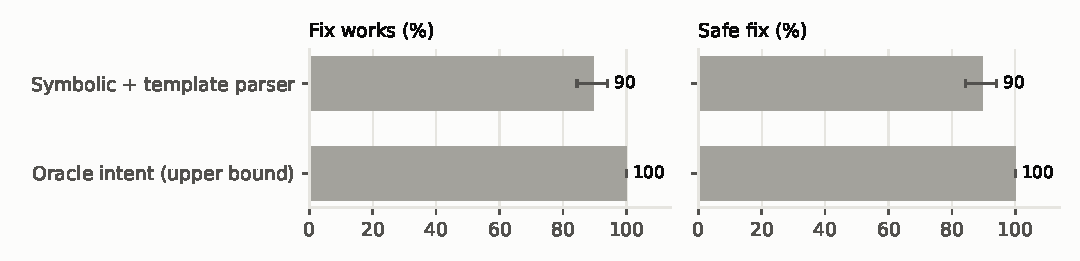
\includegraphics[width=\columnwidth]{../results/figures/fix_rates_core.pdf}
\caption{Fix-works and safe-fix rates with 95\% bootstrap intervals on the core set.}\label{fig:rates}
\end{figure}

\textbf{RQ1: Does verified diagnosis beat LLM diagnosis?} \Cref{tab:main} reports RCA@1 of \CMRcaOne{} for \sys{} (7B) versus
\LLMOnlyRcaOne{} (LLM only) and \LLMCheckRcaOne{} (with checklist). \todo{interpret once all runs finish: where each system fails, per family and level (breakdown table), McNemar p-values.}

\textbf{RQ2: Are the fixes safe?} \sys{} fixes \CMFix{} of tickets and \CMSafe{} safely; the strongest LLM baseline reaches
\LLMVerifySafe{} safe fixes, and \LLMCheckOverPriv{} of the checklist baseline's tickets are closed with an over-privileged fix.
\todo{discuss typical over-privileged edits from excess\_examples.}

\textbf{RQ3: Which components matter?} Removing the least-privilege cost (\CMNoLPSafe{} safe) isolates the repair objective;
the 3B model (\CMSmallSafe{} versus \LLMCheckSmallSafe{}) tests whether the design lets smaller models compete; the oracle
(\OracleSafe{}) bounds the loss due to intent extraction (\CMIntent{} exact intents). \todo{interpret.}

\textbf{RQ4: Are the models faithful to AWS?} The IAM model agrees with the AWS policy simulator on \IamFidelity{} of
\IamFidelityN{} random identity, boundary and resource-policy cases, and the network model with live probes on AWS in
\LiveFidelity{} of \LiveFidelityN{} probe groups covering stateful versus stateless filtering, rule order, partial ephemeral
coverage, security-group references, refused versus timed-out connections and same-subnet NACL bypass. \todo{discuss disagreements.}

\section{Threats to Validity}
\textbf{Synthetic tickets.} Tickets come from templates; real tickets are messier. The template parser exploits their
regularity, which is why it is a baseline and not our method; the LLM components never see a template. A study on real or
human-written tickets is future work.
\textbf{Circularity.} The same models that \sys{} reasons with also simulate the symptoms. Labels do not depend on them
(they come from the operators), and the fidelity experiments bound the gap between the models and AWS, but the oracle row is an
upper bound of a system whose model is perfect, not of reality.
\textbf{Scope.} The models cover a documented subset of AWS behaviour (no transit gateways, load balancers, IPv6, policy
variables); faults outside it are invisible to \sys{} but not necessarily to an LLM.
\textbf{Metric.} Excess privilege is computed over a finite universe and is a lower bound; weights in the repair cost were set
once and not tuned on test data.
\textbf{Models.} One open model family at two sizes; larger or proprietary models may close part of the gap.

\section{Conclusion}
Letting an LLM do only what it is good at, turning a ticket into a formal intent, and leaving diagnosis and repair to verified
reasoning yields fixes that are both correct and minimal on a small local model. The excess-privilege metric makes
``closed the ticket without weakening security'' measurable, and we hope \bench{} encourages evaluating troubleshooting
assistants on the safety of their fixes and not only on their answers.

\bibliographystyle{IEEEtran}
\bibliography{refs}
\end{document}
